\documentclass[table,usenames,dvipsnames]{beamer}

\usepackage[croatian]{babel}
\usepackage[utf8]{inputenc}
\usepackage{listings}
\usepackage{datetime}
\usepackage{graphics}
\usepackage{fancybox}
\usepackage{color}
\usepackage[normalem]{ulem}
\usepackage{tikz}
\usepackage{listings}
\usetikzlibrary{shapes,arrows}
\usetheme{CambridgeUS}
\usecolortheme{seagull}

\DefineNamedColor{named}{Purple}{cmyk}{0.52,0.97,0,0.55}
\setbeamertemplate{itemize item}[triangle]
\setbeamercolor{title}{fg=Purple}
\setbeamercolor{frametitle}{fg=Purple}
\setbeamercolor{itemize item}{fg=Purple}
\setbeamercolor{section number projected}{bg=Purple,fg=white}
\setbeamercolor{subsection number projected}{bg=Purple}

\setbeamertemplate{caption}{\raggedright\insertcaption\par}

\renewcommand{\dateseparator}{.}
\newcommand{\todayiso}{\twodigit\day \dateseparator \twodigit\month \dateseparator \the\year}
\newcommand{\shell}[1]{\texttt{#1}}
\definecolor{LightGray}{gray}{0.9}

\title{Osnove korištenja operacijskog sustava Linux}
\subtitle{09. Linux u praksi}
\author[Dominik Barbarić]{Dominik Barbarić\\ \small{Nositelj: dr. sc. Stjepan Groš}}
\institute[FER]{Sveučilište u Zagrebu \\
	Fakultet elektrotehnike i računarstva}

\date{\todayiso}

\begin{document}
%\beamerdefaultoverlayspecification{<+->}
{
	\setbeamertemplate{headline}[] % still there but empty
	\setbeamertemplate{footline}{}
	
	\begin{frame}
		\maketitle
	\end{frame}
}

\section{Varijable okruženja}
\begin{frame}[t]
	\frametitle{Varijable okruženja}
	\begin{itemize}
		\item Varijable okruženja (engl. \emph{environment variables}) su varijable sustava kojima mogu pristupiti svi procesi
		\item Obično se koriste za spremanje adrese nekih bitnih lokacija (korisnički direktorij, direktorij s izvršnim datotekama instaliranih programa, \ldots)
		\item[]
		\item U \shell{bash} ljusci definiraju se:
		\item[] \shell{varijabla=vrijednost}
		\item Dohvaćaju se s \$ operatorom:
		\item[] \shell{echo \$varijabla}
		\item Popis svih varijabli okruženja: \shell{printenv}
	\end{itemize}
\end{frame}

\begin{frame}[t]
	\frametitle{Varijable okruženja}
	\begin{itemize}
		\item Definiranjem varijable učinili smo je dostupnim \textbf{samo} u procesu ljuske
		\item Naredbom \shell{export} učinili smo je dostupnom svim \emph{dječijim procesima te ljuske}
		\item[] \shell{export varijabla}
		\item[\textcolor{black}{ili}] \shell{export varijabla=vrijednost}
		\item[]
		\item Za trajno "spremanje" varijable potrebno je naredbu \shell{export} staviti u neku od login skripti
		\item[]
		\item Za pokretanje programa sa zadanim varijablama okruženja možemo koristiti naredbu \shell{env}
	\end{itemize}
\end{frame}

\begin{frame}[t]
	\frametitle{Varijable okruženja}
	\framesubtitle{PATH}
	\begin{itemize}
		\item \shell{PATH} je vrlo bitna i često korištena varijbla okruženja
		\item Sadrži apsolutne adrese svih direktorija u kojima ljuska \emph{traži unesene naredbe}
		\item Adrese su odvojene dvotočjem
		\item Uobičajena vrijednost PATH varijable:
		\item[]	\small \shell{/usr/local/sbin:/usr/local/bin:/usr/sbin:/usr/bin:/sbin:/bin}
		\item[]
		\item Primjer: Pri pokretanju naredbe
		\item[] \shell{vim}
		\item[] ljuska pretražuje, redom, sve direktorije upisane u \shell{\$PATH} i pokreće prvu pronađenu izvršnu datoteku s imenom \shell{vim}
	\end{itemize}
\end{frame}

\section{Programi u Linuxu}
\begin{frame}[t]
	\frametitle{Programi u Linuxu}
	\begin{itemize}
		\item Izvršne datoteke u Linuxu mogu biti u formatu:
		\begin{itemize}
			\item \emph{a.out} - do kernela 1.2
			\item \emph{elf} (Executable and Linkable Format) - od kernela 1.2 nadalje
		\end{itemize}
		\item[]
		\item Uobičajene metode instalacije programa:
		\begin{itemize}
			\item Iz izvornog koda (tarball arhiva i \emph{make} alat)
			\item Pomoću sustava upravljanja paketima
		\end{itemize}
	\end{itemize}
\end{frame}

\begin{frame}[t]
	\frametitle{Programi u Linuxu}
	\framesubtitle{Kompajliranje i instalacija}
	Zašto instaliravati programe iz izvornog koda?
	\begin{itemize}
		\item Linux je multiplatformski OS
		\item Izvorni kod je pisan za određeni OS (ne ovisi o arhitekturi, osim u programima posebne namjene)
		\item Kompajliranjem izvornog koda na odredišnoj arhitekturi dobivamo valjanu izvršnu datoteku
		\item[]
	\end{itemize}
	Distribucija izvornih kodova open source programa
	\begin{itemize}
		\item Većina izvornih kodova open source programa pisanih za Linux dolaze u tar arhivama
		\item Tar arhive se obično dodatno komprimiraju gzip kompresijskim formatom - \emph{tarball} (.tar.gz / .tgz)
	\end{itemize}
\end{frame}


\begin{frame}[t]
	\frametitle{Programi u Linuxu}
	\framesubtitle{Kompajliranje i instalacija}
	\emph{make}
	\begin{itemize}
		\item Alat koji služi za automatizaciju kompajliranja i instalacije programa
		\item[] Sintaksa: \shell{make <target>}
		\item \shell{make} se oslanja na skriptu \shell{Makefile} koja se nalazi u direktoriju s izvornim kodom
		\item \shell{make} izvršava \emph{target} (ciljni) posao definiran u Makefileu
		\item[]
		\item Za svaki projekt piše se specifični Makefile koji onda izvršava sve potrebne radnje koje omogućuju kompajliranje i/ili instalaciju i pokretanje programa (npr. instaliranje posebnih bibilioteka, \ldots)
		\item Uobičajeni targeti u Makefileu su \emph{all}, \emph{install}, a mogu se definirati i targeti za deinstalaciju programa
	\end{itemize}
\end{frame}

\subsection{Sustavi upravljanja paketima}
\begin{frame}[t]
	\frametitle{Programi u Linuxu}
	\framesubtitle{Sustav upravljanja paketima}
	\begin{itemize}
		\item Programski paketi se u većini distribucija instaliraju \emph{sustavom upravljanja paketima}
		\item Programi dolaze u paketima u kojima se nalaze izvorni kod ili (češće) izvršni program te podaci o koracima koje je potrebno provesti za instalaciju i pokretanje programa - \emph{dependencies}
		\item Sustav upravljanja paketima pamti instalirane pakete te vodi računa o ažuriranju i postupcima za deinstalaciju paketa
	\end{itemize}
\end{frame}

\begin{frame}[t]
	\frametitle{Programi u Linuxu}
	\framesubtitle{Sustavi upravljanja paketima}
	Poznatiji sustavi upravljanja paketima:
	\begin{table}[h]
		\rowcolors{1}{White}{LightGray}
		\begin{tabular}{l l l}
			\rowcolor{BlueViolet!20} Sustav & Distribucije & Format paketa \\
			dpkg & Debian, Ubuntu, Knoppix, ... & .deb \\
			RPM & Red Hat, Fedora, openSUSE, Cent OS, ... & .rpm \\
			pacman & Arch & .tar.xz \\
		\end{tabular}
	\end{table}
	\begin{itemize}
		\item Svaki od ovih sustava se može koristiti pomoću ugrađenih alata ili putem nekog \emph{frontenda}
		\item Primjer - Debian
		\item[] \shell{apt-get install vim}
		\item[] \small Naredba poziva \emph{apt} (Advanced packaging tool - frontend za dpkg) koji pretražuje Debianov repozitorij te preuzima i instalira paket \shell{vim}
	\end{itemize}
\end{frame}

\begin{frame}[t]
	\frametitle{Programi u Linuxu}
	\framesubtitle{Sustavi upravljanja paketima}
	\begin{itemize}
		\item \shell{apt} je frontend za \shell{dpkg}
		\begin{itemize}
			\item Spaja se s Debian / Ubuntu / \ldots repozitorijima navedenim u
			\item[] \shell{/etc/apt/sources.list}
			\item Vodi računa o redovitom ažuriranju instaliranih paketa
			\item Za apt postoje i napredniji frontendi (npr. \emph{Synaptic package manager}, \shell{aptitude}, \ldots)
		\end{itemize}
		\item \shell{dpkg} se može koristiti kao samostalan alat za instalaciju lokalno dostupnih .deb paketa
		\item[]
		\item Zadatak
		\begin{itemize}
			\item Proučiti man stranice za dpkg i isprobati ručnu instalaciju nekog paketa iz službenog repozitorija distribucije
		\end{itemize}
	\end{itemize}
\end{frame}

\section{Grafičko korisničko sučelje}
\begin{frame}[t]
	\frametitle{Grafičko korisničko sučelje}
	\begin{itemize}
		\item GUI je u većini UNIX sustava ostvaren pomoću sustava \emph{X Window System}
		\begin{itemize}
			\item Najpoznatija implementacija X sustava je \emph{Xorg} koji koristi \emph{X11} protokol X sustava
			\item Xorg je serverska aplikacija koja omoućuje prikaz grafičkih elemenata na zaslonu
			\item X sustav omogućuje i mrežno korištenje grafičkih aplikacija (pokrenutih na udaljenom serveru)
		\end{itemize}
		\item Window managers
		\begin{itemize}
			\item Koriste X sustav za crtanje prozora i \textit{ukrase} prozora (naslovna traka, izbornici, scroll bar, \ldots)
			\item[]
			\item Primjeri najčešće korištenih window managera:
			\item[] Metacity, Xfwm, Kwin, Compiz, Mutter, Openbox, twm, \ldots
		\end{itemize}
	\end{itemize}
\end{frame}

\begin{frame}[t]
	\frametitle{Grafičko korisničko sučelje}
	\framesubtitle{Xorg s twm window managerom}
	\centering 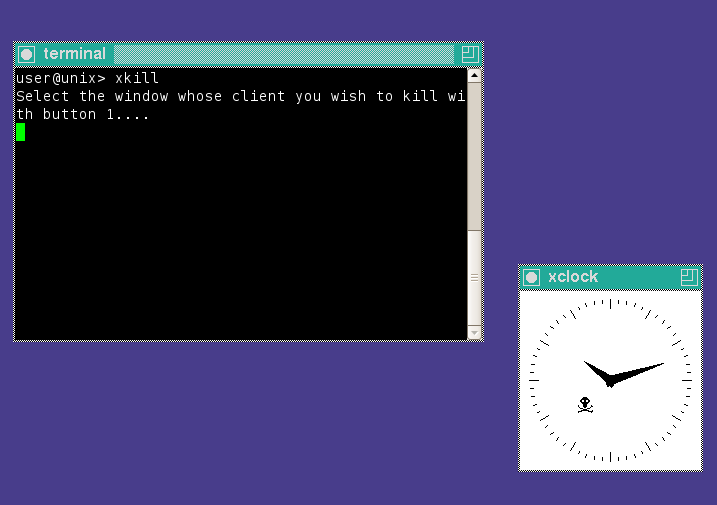
\includegraphics[width=270pt]{xorg.png}
\end{frame}

\begin{frame}[t]
	\frametitle{Grafičko korisničko sučelje}
	\begin{itemize}
		\item \emph{Grafičke ljuske} (engl. \emph{Graphical shells})
		\begin{itemize}
			\item Koriste window manager za prikaz ljuske
			\item Omogućuju prikaz kompletnog grafičkog sučelja
			\item Uvodi funkcionalnosti pokretanja programa iz GUI-a, bolje upravljanje prozorima i radnim površinama
		\end{itemize}
		\item \emph{Desktop environment}
		\begin{itemize}
			\item Predstavlja kompletno rješenje grafičkog korisničkog sučelja
			\item U mnogim distribucijama dolazi neki predinstalirani desktop environment
			\item Mogu se po volji mijenjati; Ponovnom instalacijom ili odabirom između više instaliranih desktop environmenta pri loginu
			\item[]
			\item Primjeri najpoznatijih desktop environmenta:
			\item[] Gnome, KDE, Xfce, Unity, MATE, Cinnamon, \ldots
		\end{itemize}
	\end{itemize}
\end{frame}

\begin{frame}[t]
	\frametitle{Grafičko korisničko sučelje}
	\framesubtitle{Gnome 3}
	\centering 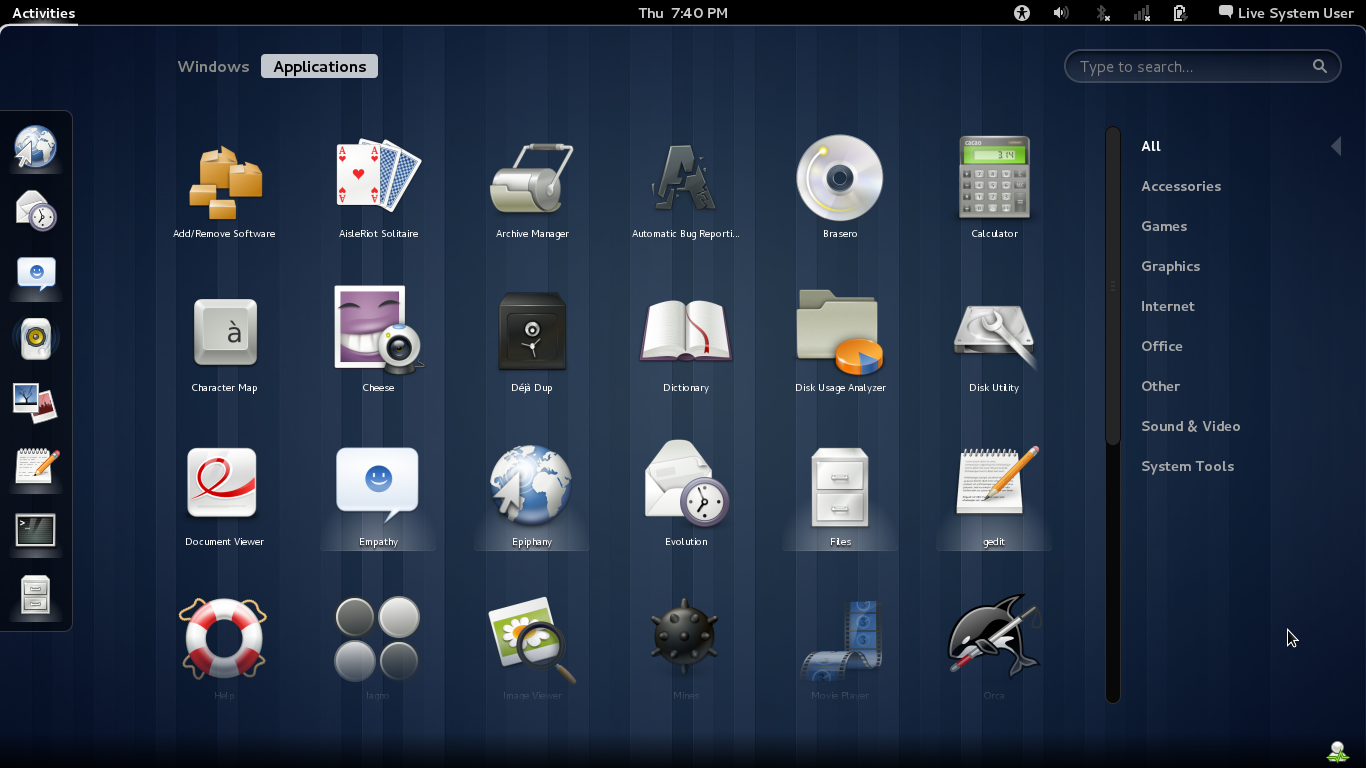
\includegraphics[width=0.95\textwidth]{gnome3.png}
\end{frame}

\begin{frame}[t]
	\frametitle{Grafičko korisničko sučelje}
	\begin{itemize}
		\item Kao dio GUI-a se obično instalira i \emph{Login manager}
		\begin{itemize}
			\item Početni login zaslon
			\item Omogućuje automatsku ili korisničku prijavu na sustav
			\item Omogućuje odabir desktop environmenta
		\end{itemize}
		\item Login manageri često dolaze u paketu s desktop environmentima
	\end{itemize}
\end{frame}

\begin{frame}[t]
	\frametitle{Mreža}
	\begin{itemize}
		\item UNIX je kao višekorisnički operativni sustav predstavljao osnovu za izgradnju današnjih računalnih mreža
		\item Mnogo aplikacija se temelji na server-klijent arhitekturi
		\begin{itemize}
			\item Mogućnost udaljenog rada
		\end{itemize}
		\item[]
		\item Računala se umrežavaju putem mrežnih sučelja
		\item Za mrežna sučelja u Linuxu najčešće susrećemo oznake:
		\begin{itemize}
			\item Za žičana \emph{ethernet} sučelja - \shell{eth0}, \shell{eno1}, \shell{enp1s0}, \ldots
			\item Za bežična \emph{WLAN} sučelja - \shell{wl0}, \shell{wifi0}, \ldots
			\item Za \emph{loopback} sučelje - \shell{lo}
		\end{itemize}
	\end{itemize}
\end{frame}

\begin{frame}[t]
	\frametitle{Mreža}
	\framesubtitle{Podešavanje pristupa mreži}
	\begin{itemize}
		\item Za podešavanje TCP/IP postavki koriste se \shell{ifconfig} i \shell{route}
		\begin{itemize}
			\item U novijim distribucijama ove naredbe su objedinjene naredbom \shell{ip}
		\end{itemize}
		\item Konfiguracija postavljena ovim naredbama je privremena i bit će zaboravljena nakon restarta
		\item Pri startupu (pokretanju \shell{networking} servisa) konfiguracija se čita iz \shell{/etc/network/interfaces}
		\begin{itemize}
			\item Ponovno učitavanje postavki iz \shell{/etc/network/interfaces} se tijekom rada može pozvati restartom mrežnog servisa:
			\item[] \shell{/etc/init.d/networking restart}
		\end{itemize}
		\item[]
		\item Kod bežičnih mreža se računalo treba asocirati s mrežom prije TCP/IP konfiguracije
		\begin{itemize}
			\item Najčešće korišteni alati: \shell{iwconfig}, \shell{iw}
			\item Za WPA enkripciju još i \shell{wpa\_supplicant}
		\end{itemize}
	\end{itemize}
\end{frame}

\begin{frame}[fragile]
	\frametitle{Podešavanje pristupa mreži}
	\framesubtitle{Primjer podešavanja mreže}
	\begin{block}{/etc/network/interfaces}
		\ttfamily
		\begin{verbatim}
		auto eth0
		iface eth0 inet static
		address 192.168.1.5
		netmask 255.255.255.0
		gateway 192.168.1.254
		
		auto eth1
		iface eth1 inet dhcp
		\end{verbatim}
	\end{block}
	\begin{itemize}
		\item \shell{auto eth0} - \shell{eth0} se omogućuje pri startupu
		\item \shell{iface eth0 inet static} - \shell{eth0} ima dodijeljenu statičku IP adresu
		\item \shell{iface eth1 inet dhcp} - \shell{eth1} traži dinamičku IP adresu
	\end{itemize}
\end{frame}

\begin{frame}[t]
	\frametitle{Podešavanje pristupa mreži}
	\framesubtitle{Pregled naredbi}
	\begin{table}[h]
		\rowcolors{1}{White}{LightGray}
		\begin{tabular}{p{4cm} p{3cm} p{3cm}}
			\rowcolor{BlueViolet!20}Operacija & \shell{ifconfig} & \shell{ip} \\
			Pregled konfiguracije & \shell{ifconfig} & \shell{ip addr show} \\ & & \shell{ip link show} \\
			Uključenje i isključenje sučelja & \shell{ifconfig <interface> up|down} & \shell{ip link set <interface> up|down} \\
			Podešavanje IP adrese & \shell{ifconfig <interface> <IP>} & \shell{ip address add|del <IP> dev <interface>} \\
			Pregled ruta & \shell{route} & \shell{ip route show}
		\end{tabular}
	\end{table}
\end{frame}

\begin{frame}[t]
	\frametitle{Mreža}
	\framesubtitle{Podešavanje pristupa mreži}
	\begin{itemize}
		\item Kod većine novih distribucija na sustav dolazi predinstaliran alat \emph{Network manager}
		\item Network manager za konfiguraciju \textbf{ne koristi} datoteke i alate koje smo dosad opisali
		\begin{itemize}
			\item U datoteci \shell{/etc/network/interface} se \emph{ne smiju} navoditi sučelja koja konfiguriramo kroz Network manager može doći do konflikta
		\end{itemize}
		\item Network manager je namijenjen korištenju iz grafičkog sučelja
		\begin{itemize}
			\item User friendly konfiguracija mreže
		\end{itemize}
		\item Kroz dodatne module Network manager podržava razne vrste mreža {\small (PPTP, GPRS/UMTS, ADSL, WiMAX, Bluetooth, Dial up, \ldots)}
	\end{itemize}
\end{frame}

\begin{frame}[t]
	\frametitle{Podešavanje pristupa mreži}
	\framesubtitle{Network manager}

	\begin{figure}[h]
		\begin{minipage}{0.4\textwidth}
			\centering
			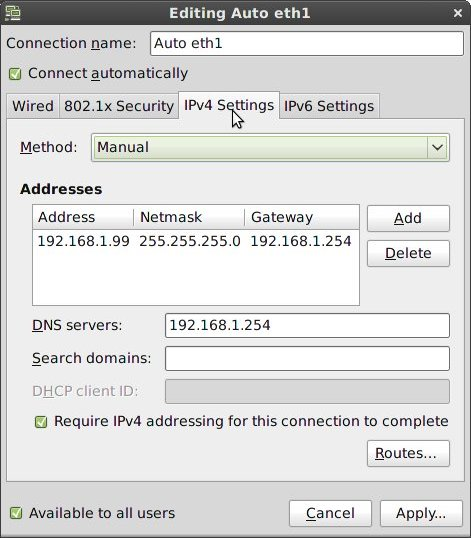
\includegraphics[width=\linewidth]{nm-ethernet.jpg}
			\caption{Konfiguracija IP adrese}
		\end{minipage}
		\begin{minipage}{0.45\textwidth}
			\centering
			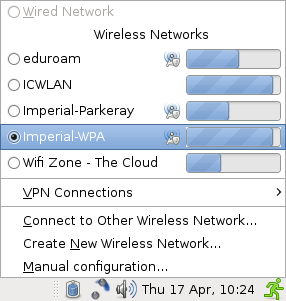
\includegraphics[width=0.8\linewidth]{nm-applet.png}
			\caption{Odabir WLAN mreže}
		\end{minipage}
	\end{figure}
\end{frame}	

\begin{frame}[t]
	\frametitle{Literatura}
	man stranice: \shell{a.out}, \shell{elf}, \shell{tar}, \shell{make}, \shell{dpkg}, \shell{ifconfig}, \shell{ip}, \shell{interfaces}
	
	\begin{itemize}
		\item \url{http://cs.mipt.ru/docs/comp/eng/os/linux/howto/howto\_english/elf/elf-howto-1.html}
		\item \url{http://www.opensourceforu.com/2012/06/gnu-make-in-detail-for-beginners/}
		\item \url{http://www.rpm.org/max-rpm/ch-intro-to-rpm.html}
		\item \url{http://structbio.vanderbilt.edu/comp/unix/part03.php}
		\item \url{http://docbook.rasip.fer.hr/ddb/public/index.php/publication/html/rasipbook/id/1?chapter=4.1&rce=0&tts=0&css=original&edit=0}
		\item \url{http://www.tty1.net/blog/2010/ifconfig-ip-comparison_en.html}
	\end{itemize}
\end{frame}
	
\end{document}